\part{De l’expertise archivistique à la formalisation d’un traitement automatisé}

\chapter{Cartographie, caractéristique et caractérisation technique des archives numérique d’exposition}

Le traitement des documents d'un vaste corpus nécessite dans un premier temps une connaissance de leur composition. Nous avons relevé que les archives d'exposition sont le résultat de la mission de service public confié au musée. De ce fait, leur structuration est primordial, une obligation légale pour le service en charge des archives comme pour les autres services producteurs. Dans l'institution, les documents d'exposition parties précédentes, les documents d'exposition de l'actif se trouvent dans l'espace collaboratif Teams, tandis que ceux du passif (c'est-à-dire les dossiers d'exposition antérieurs à 2018) sont conservés sur le serveur YODA. Le serveur est organisé en sous ensemble de stockage, une partition collective par service et une partition pour production individuelle des salariés. Cette organisation engendre une structuration en plusieurs espaces de stockage. Les archives d'expositions que nous étudions dans le cadre de notre mémoire se retrouvent intégrées dans le deuxième ensemble.\\[0.1cm]

Pour se faire, notre mission à ce stade, ne consiste pas à apporter une modification à l’organisation de l'institution, mais plutôt de faire un constat de l'existant. Trois questions suscitent un intérêt: où se trouvent les archives numériques d'exposition? De quoi sont-elles techniquement constituées? Pourquoi les informations qui ressortent des interrogations ne sont-elles pas suffisantes pour leur appliquer un traitement archivistique? Deux outils nous permettent d'apporter des éléments de réponse : un sur la connaissance large des arborescences de fichiers et la prise en compte des éléments indispensables à la cartographies des documents, tells que la volumétrie ; un autre sur l'identification des formats. Le but pour nous n'est pas de faire la cartographie de tout le serveur mais plutôt d'identifier les espaces cibles contenant les documents d'exposition. 


Cette étape constitue une phase de diagnostic car les résultats obtenus apportent une description technique des fichiers du corpus des exposition et des informations sur leur environnement. Le présent chapitre se divise en trois parties. En premier lieu, l’idée est de faire une présentation de la cartographie réalisée à partir de l'outil Archifiltre. En second lieu présente les caractéristiques techniques des documents. En dernier lieu, on fait une analyse des limites de cet audit face aux besoins de structuration.


\section{Cartographie des archives d’exposition par Archifiltre}

Archifiltre est principalement conçu pour aider les archivistes à résoudre les problèmes liés au traitement des fonds numériques\footnote{\cite{beta-gouv-archifiltre}.}. Dans l'espèce, la solution se saisit du vrac tel qu'il existe, dans son organisation initiale pour lui donner une vision d'ensemble. 

\subsection*{Audit du corpus}

Lorsqu'on est confronté à un volume important de documents, peu importe le support, il est préférable de commencer par un état des lieux. Celui-ci permet d'avoir une vue d'ensemble sur le corpus à traiter. Le cas des archives numériques reste quelque fois difficile à appréhender. 
La particularité de l'audit est qu'il permet d'avoir une connaissance plus aiguisée des fichiers, leur arborescence et leur environnement. Notre audit est effectué sur la base de la version 4.2.1 de l'outil open source Archifiltre\footnote{\cite{programme-vitam-archifiltre}.}, porté par \enquote{fabrique numérique des ministères sociaux}\footnote{\cite{beta-gouv-archifiltre}} depuis 2017\footnote{\cite{programme-vitam-archifiltre}}. Il permet d'analyser et de visualiser les arborescences de  fichiers\footnote{\cite{beta-gouv-archifiltre}}. Son utilisation permet d’avoir une vue globale sur les données dont on a la charge. Dans le cadre de notre projet, l'outil sert avant tout de porte d'entrée pour comprendre le contenu et la structure des archives d'exposition. 

L'analyse est menée sur une partie du serveur YODA. Pour chaque répertoire exploité, les données issues de l'analyse sont exportées sous forme de  deux fichiers. L'audit prend une forme simple (fichier word) et l'export de la liste des fichiers et répertoires prend une forme de tableau (CVS : \textit{Comma-Separated Values}). Les exports comportent les informations sur le nom du répertoire d'archives, son emplacement et sa taille, ce qui permet de passer de la simple vue des données accessibles via l'explorateur fichiers de l'ordinateur vers un audit technique suivi d'une représentation visuelle.

Cette étape s’avère particulièrement intéressante pour notre démarche car, elle nous permet non seulement de situer les dossiers d'exposition dans le serveur YODA mais aussi de comparer les répertoires d'archives qui les comportent. À partir de là, nous pouvons déterminer la volumétrie des documents, leur quantité totale et éventuellement des anomalies. 


La consolidation des résultats obtenus permet de faire une représentation commune des différents répertoires audités. Après avoir fusionné les fichiers CSV via l'outil Excel/\textit{Power Query}, nous avons effectué un nettoyage en y ajoutant des colonnes qui répondent aux interrogations sus-évoquées. Nous sommes aussi passés par une étape intermédiaire : celle de la visualisation  par le biais de l'outil tableau. Il s'agit d'un outil de visualisation qui permet de représenter des jeux de données sous diverses apparences. La visualisation nous a permis d'avoir une vision transversale de notre corpus.

Toutefois, avec la cartographie produite, nous ne cherchons pas encore à déterminer la valeur archivistique des documents. Elle est utilisée comme un outil d'aide au diagnostic.

\vspace{-5.5cm} % Pour faire monter le texte
\subsection*{Répartition sectorielle et volumétrie des archives d’exposition}

\vspace{-1.5cm} % Pour faire monter le texte

Comme nous l'avons mentionné plus haut, l'exploitation des données nous permet dans un second temps de répondre à la question de comment sont réparties les archives du périmètre? Mieux, où se trouvent-elles? L'exploitation des données exportées permet d'identifier les différents répertoires de premier niveau dans lesquels sont conservés les documents d'exposition. Dans l'optique de rendre cette répartition lisible, nous retenons pour la présentation graphique les quinze répertoires présentant le nombre de fichiers le plus élevé. Ce choix fait ressortir les principaux espaces de stockage documentaire.

\begin{figure}[H]
	\centering
	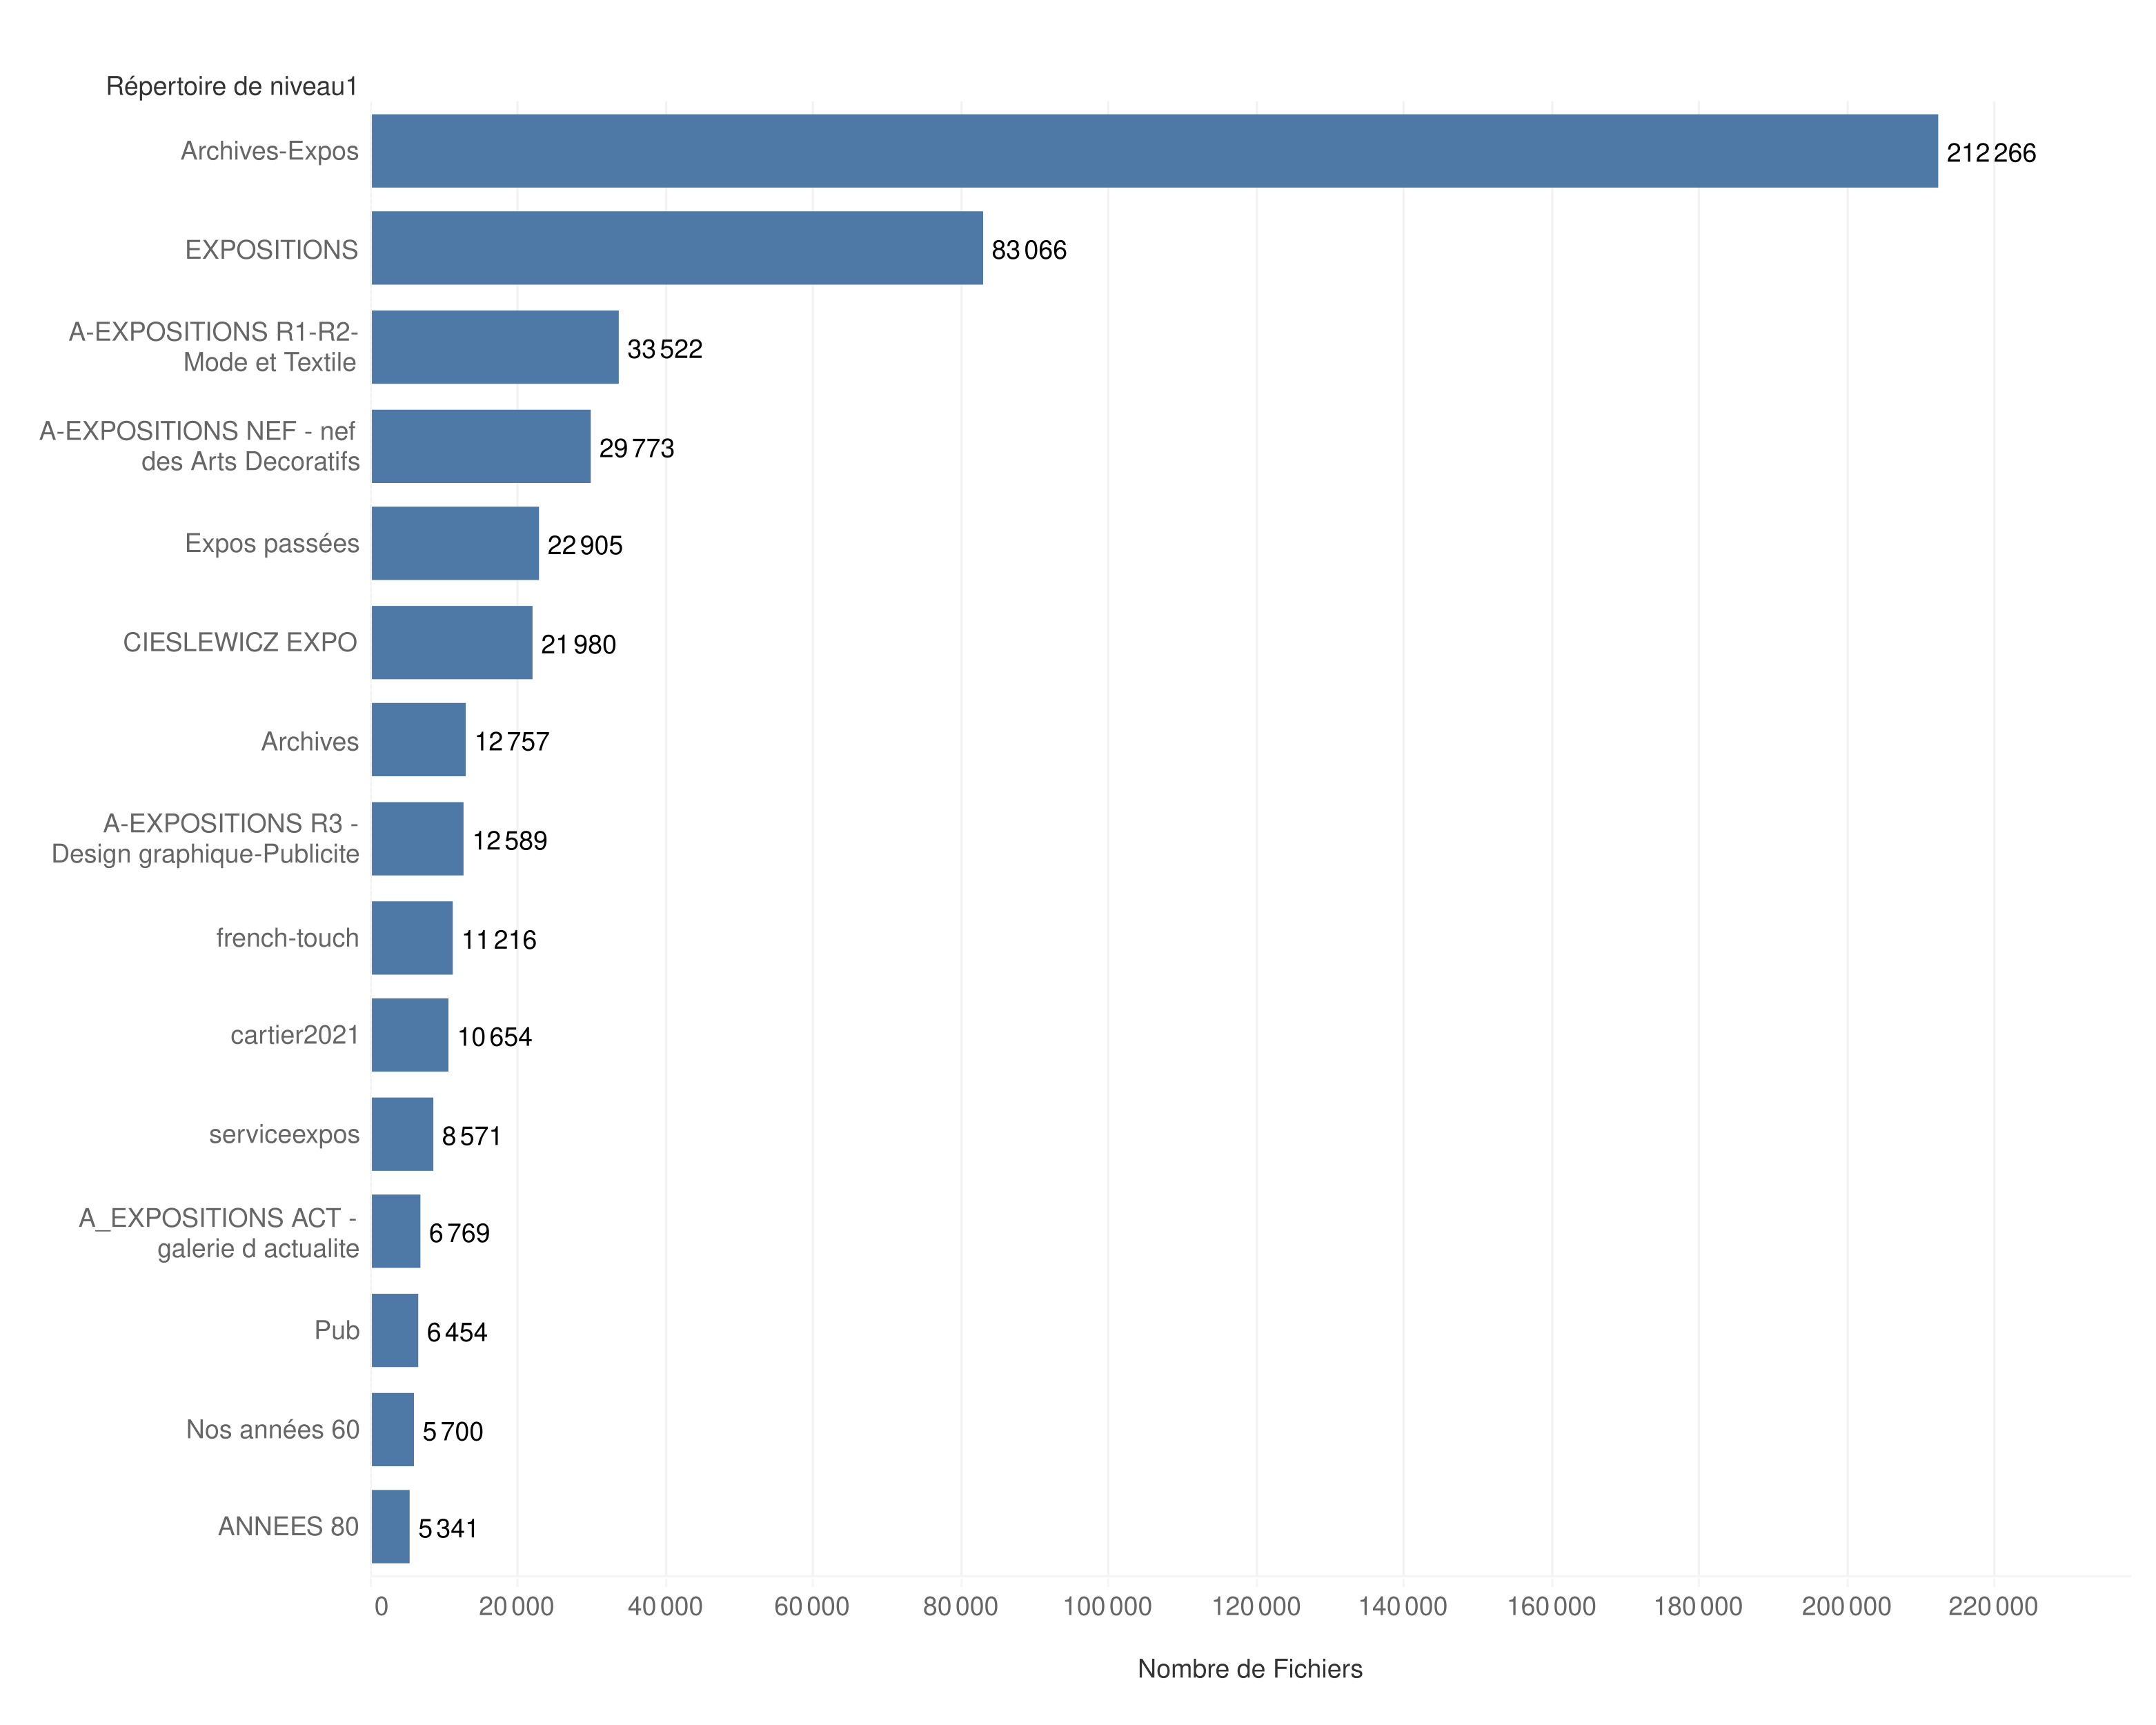
\includegraphics[width=0.9\textwidth]{Images/Repartition_15_Repertoires_Archives.png}
	\caption{Visualisation de 15 répertoires d'archives d'exposition}
	\label{fig:Repartition}
\end{figure}

Cette représentation fait apparaître une répartition inégale. Certains répertoires concentrent une part importante de fichiers, alors que d'autres sont presque vides. Cela se confirme avec les résultats du premier répertoire, \enquote{Archives-Expos} qui à lui seul totalise un nombre de 212 266 fichiers. Tandis que les autres comptent moins de la moitié de son volume. À partir de là, on observe donc une véritable concentration autour de certains espaces. Deux répertoires de même niveau hiérarchique peuvent en réalité correspondre à des masses documentaires différentes. La place qu'occupe un dossier dans l'arborescence ne peut renseigner à elle seule sur son importance quantitative. Cette analyse permet dénombre total de fichiers et leur poids : soit 553 432 pour le les fichiers et 2,43 To (téraoctets) de volumétrie totale des dossiers d'exposition compris dans les 8,43 To du serveur. 


En examinant les titres des répertoires, on observe une différence dans la logique de nommage. Certains répertoires renvoient à des espaces d'expositions (A-EXPOSITIONS NEF – nef des Arts Décoratifs,A-EXPOSITIONS R1-R2 – Mode et Textile, etc.), et d'autres à des expositions (CIESLEWICZ EXPO, french-touch, etc.). L'une des anomalies que l'audit nous permet de desceller pour comprendre un fonds.


\section{ Identification technique des fichiers du corpus}

\vspace{-0.4cm}
Au-delà de la volumétrie, la cartographie permet d'identifier les caractéristiques techniques des fichiers. Il s'agit de prendre connaissance des documents qui composent le périmètre. Le logiciel utilisé pour cette étape d'identification technique est la solution Droid-sh (\textit{Digital Record Object Identification}): il s'agit d'un outil développé par les Archives nationales britanniques, il s'appuie sur le registre PRONOM (\textit{Public Record Office and Nôm}) pour identifier les formats de fichiers à partir des signatures propres à chaque fichier. Pronom est comme une  « système d'information en ligne sur les formats de fichiers de données et leurs logiciels associés»\footnote{\cite{nationalarchives-pronom}.}.


\subsection*{Identification et diversités des formats}


L'analyse laisse voir une large diversité de formats des fichiers au sein des dossiers d'exposition. Celle-ci se justifie par la variété des activités de préparation des expositions et aux différents environnements logiciels utilisés par les producteurs. Les résultats obtenus permettent non seulement de faire une répartition par famille de formats, mais aussi d'identifier les formats prépondérants et plus largement de détecter d'éventuelles anomalies.

\begin{figure}[H]
	\centering
	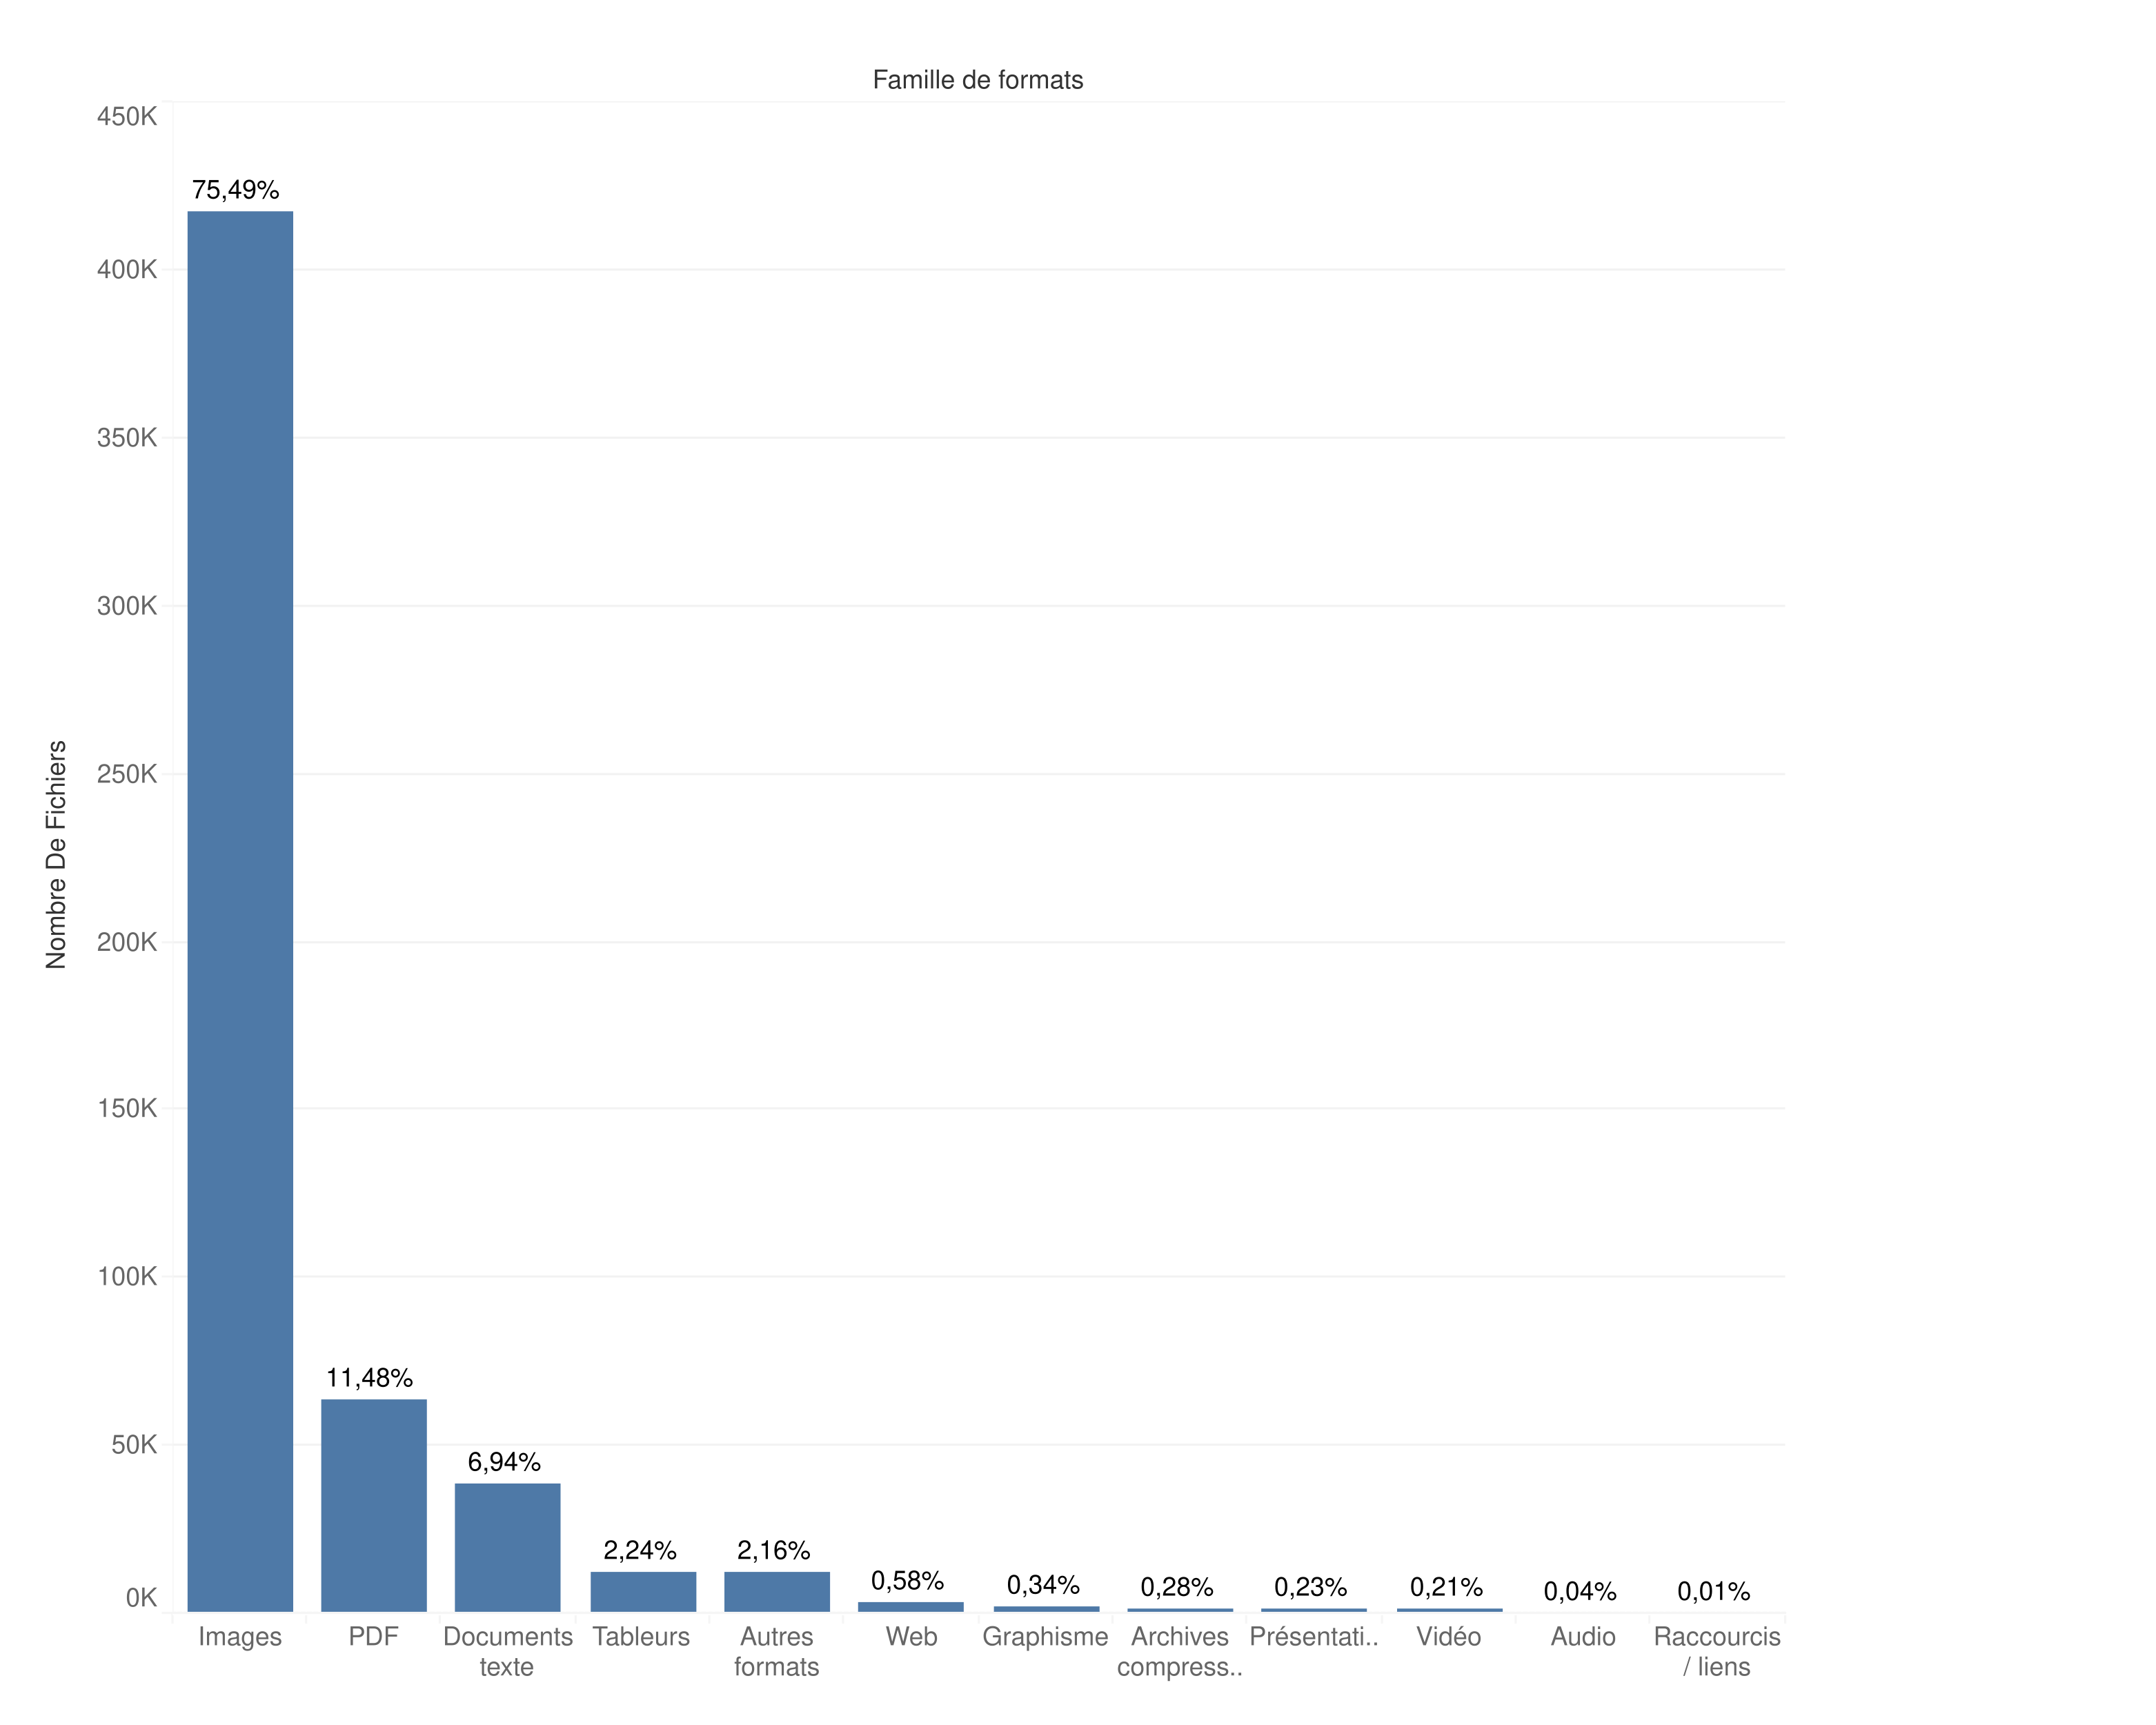
\includegraphics[width=0.8\textwidth]{Images/Repartition-Famille-Formats.png}
	\caption{Répartition des familles de formats de fichiers}
	\label{fig:Repartition-famille-formats}
\end{figure}

\begin{table}[H]
	\centering
	\renewcommand{\arraystretch}{0.5}
	\setlength{\tabcolsep}{3 pt}
	\resizebox{\textwidth}{!}{%
		\begin{tabular}{lrr}
			\toprule
			\textbf{Famille de formats} & \textbf{Nombre de fichiers} & \textbf{Pourcentage (\%)} \\
			\midrule
			Images                 & 417~782 & 75,49~\% \\
			PDF                    & 63~527  & 11,48~\% \\
			Documents texte        & 38~382  & 6,94~\% \\
			Tableurs               & 12~418  & 2,24~\% \\
			Autres formats         & 11~961  & 2,16~\% \\
			Web                    & 3~202   & 0,58~\% \\
			Graphisme              & 1~906   & 0,34~\% \\
			Archives compressées   & 1~554   & 0,28~\% \\
			Présentations          & 1~254   & 0,23~\% \\
			Vidéo                  & 1~156   & 0,21~\% \\
			Audio                  & 241     & 0,04~\% \\
			Raccourcis             & 49      & 0,01~\% \\
			\midrule
			\textbf{Total}         & \textbf{553~432} & \textbf{100,00~\%} \\
			\bottomrule
		\end{tabular}%
	}
	\caption{Répartition des fichiers du fonds par famille de formats}
	\label{tab:repartition_formats}
\end{table}

\vspace{0.5cm} % Renvoyer la ligne vers le bas	
À l'issue de l'analyse, douze familles sont identifiées au sein du fonds (voir figure~\ref{fig:Repartition-famille-formats} et tableau~\ref{tab:repartition_formats}). On observe une prédominance fulgurante des formats d'image, qui représentent à eux seuls trois quarts du volume total (75,49 \%, pour 417 782 fichiers). Les documents de gestion et de travail (PDF et documents bureautiques) représentent le second ensemble le plus représenté, tandis que les formats multimédias (images, video) et de conception graphique sont minoritaires. Les autres autres formats listés font référence aux extensions qui n'existent pas : .Administration, .graphe, .adéfinir, .service, etc. Ces extensions sont la conséquence d’un mauvais nommage qui comporte un point à la place d'un \textit{underscore} et qui résultent de l'activité métier. En effet, l'outil identifie comme extension tout ce qui suit un point. 

\subsection*{Empreinte numériques et identification des fichiers identiques}

Comme l'a montrée l'étude du vrac dans les chapitres précédents, la coexistence de plusieurs occurrences d'un fichier dans différents emplacements est dû aux modalités de travail et de stockage. Le but de l'audit ici est de pointer cette anomalie à partir d'une analyse globale.

L'empreinte numérique constitue une forme d'identifiant unique qui permettant de repérer un fichier dans un ensemble. À l'image du NIR (numéro d'inscription au répertoire de la sécurité sociale), encore appelé \enquote{numéro de sécurité sociale}, qui permet d'identifier une personne dans le système de protection sociale français, l'empreinte numérique permet de distinguer un fichier d'un autre. À cet égard, il devient important de le générer. Nous choisissons de le faire avec Droid-sh qui le faire, il calcule automatiquement à partir du contenu d'un document. Toute modification du contenu affecte le calcul, donc modifie l'empreinte. Le logiciel identifie le nombre d’occurrence des fichiers à partir de l'empreinte, indépendamment de leur nom d'origine. C'est ce qu'on appelle des fichiers identiques, les doublons. Cette notion se distingue des versions des documents ( qui représentent différentes mises à jour effectuées sur un document tout au long de son cycle de vie). 



\section{Les limites de l’audit technique face aux besoins de structuration}


L'utilisation de solutions gratuites, telles qu'Archifiltre et DROID pour la réalisation d'un audit met en lumière plusieurs aspects : l'emplacement exacte des archives d'exposition dans le serveur, leur volumétrie, leur format ainsi que leur place dans le serveur par rapport aux autres documents qui s'y trouvent. 

Même si l'audit occupe une place importante dans le processus de prise en charge d'un vrac numérique, il ne permet pas à lui seul le traitement archivistique que nous souhaitons réaliser.


\subsection*{Une identification des documents insuffisante pour leur qualification}

Le document numérique se positionne au même niveau que le document papier, c'est ce que souligne Code Civil dans son article 1366. Il mentionne que :\enquote{L'écrit électronique a la même force probante que l'écrit sur support papier, sous réserve que puisse être dûment identifiée la personne dont il émane et qu'il soit établi et conservé dans des conditions de nature à en garantir l'intégrité}\footnote{\cite{code-civil-1366}}. Comme nous l'avons mentionné plus haut, l'audit se présente comme une sorte de \enquote{carte géographique} de l'arborescence fichier à traiter, il détermine avec précision les différents endroits dans lesquels on retrouve les documents, indique la place qu'ils prennent et repère les chemins d'accès. Malgré cette vision, plusieurs points ne facilitent pas leur qualification intellectuelle et juridique.

\textbf{La limite des métadonnées techniques }  Les résultats de l'audit technique seuls ne permettent pas de qualifier juridiquement et intellectuellement les documents. En effet, le scan identifie les informations techniques telles que le format de fichiers (.pdf, .jpg, .tiff), la taille ou les dates d'enregistrement et de modification. Ces éléments ne permettent pas de déterminer la valeur de preuve d'un document (un document enregistré : Cartel-salle6, ne renseigne pas sur son importance ou sur l'obligation légale de conservation).

\textbf{Le problème de la corruption sémantique}  Le problème de nommage n'est pas le résultat d'un mauvais travail de l'archiviste, mais plutôt le résultat des pratiques non encadrées. Un fichier mal nommé rend difficile son identification mais aussi la fonctionnalité de nommage intégrée aux outils d'audit (Archifiltre). On se retrouve face à des titres non signifiant c'est-à-dire flous, avec des abréviations métiers ou des noms propres des salariés. Avec la masse importante que représente le vrac, il est primordial d'effectuer un vrai travail de contrôle après cette opération. 


\subsection*{L’absence de structuration documentaire exploitable}

En effet, en dehors de la qualification des documents, l'audit ne répond pas à une organisation du fonds. Le scan fournit est le résultat de la photographie de l'arborescence des services, celle-ci découle des pratiques quotidiennes des collaborateurs. Il résulte de là une organisation souvent anarchique et non structurée; pourquoi? Parce que leur méthode de rangement n'est pas conforme aux exigences du plan de classement de l'institution. Cette situation montre la limite des solutions utilisées, car elles ne permettent pas de créer l'arborescence métier et de ranger les documents en fonction de leur contexte.



\chapter{Développement et modélisation des solutions techniques en Python}

Une fois le corpus connu, et l'identification des caractéristiques techniques effective, on peut se demander comment faire pour rendre le vrac exploitable. C'est la question à laquelle nous avons essayé de répondre durant notre alternance au MAD. Nous avons proposé une solution, puis nous l'avons expérimenté sur un ensemble concret. Pour ce faire, nous avons conçu un prototype algorithmique qui se décline en trois phases, et basé sur des actions concrètes à partir du langage de programmation Python. 
Ce chapitre se donne donc l'objectif de présenter la chaîne de traitement du vrac numérique telle que nous l'avons proposé, d'abord une intervention sur la structure matérielle des documents dans le but de rendre accessible le contenu compressé, ensuite le tri préalable des documents par catégories, enfin leur transfert vers l'arborescence de  fichiers.

\section{Préparation des données : automatiser la décompression des fichiers}

Avant d'effectuer le traitement des dossiers d'exposition, nous avons, à partir des résultats de l'audit technique Archifiltre remarqué la présence de documents compressés. Or, il est important d'accéder à tous les documents pour garantir un traitement efficace.

\subsection*{La décompression comme préalable au traitement du fonds}

Le traitement des données, structurées ou en vrac ne peut s'opérer directement sur des données encapsulées, comme les archives compressées. La décompression ici constitue l'étape préliminaire au traitement, dans le sens où elle nous donne accès à l'ensemble des documents qu'il contient. Cette opération représente une ouverture au tri des documents : si ceux-ci ne sont pas accessibles dans leur intégralité, alors le fonds en lui-même demeure partiellement inaccessible, ce qui rend difficile le traitement. Loin d'avoir du sens uniquement dans le contexte informatique, la décompression est abordée dans le contexte archivistique. C'est ce qu'illustre la norme \textit{Preservation Metadata} : \textit{Implementation Strategies} (PREMIS) dans son vocabulaire, elle la qualifie comme le processus qui consiste à inverser les effets de la compression\footnote{\cite{loc_premis_decompression}}. En d'autres termes, c'est l'action qui donne accès aux contenus des fichiers compris dans les dossiers archives. On se rend donc compte que la décompression, même si elle ne constitue pas un traitement archivistique. Dans le cadre de notre expérimentation, elle est considérée comme une opération préalable — une réflexion matérialisée en amont pour la suite du traitement.


\subsection*{Conception du script et contrôle des opérations de décompression}

Avant d'entrer dans le vif du sujet, il convient de mentionner que les résultats d'Archifiltre mettent en évidence cinq extensions d'archives compressées dans le corpus, à savoir : .zip, .rar, .7z, .tar et .gz. L'objectif est donc d'identifier ces archives et d'extraire d'elles le contenu informationnel qu'elles comportent. Afin de matérialiser cet impératif de préparation, nous avons conçu un script Python. Il effectue le traitement de manière sécurisée sur un ensemble important de documents.
Son exécution repose sur trois actions majeures, en respectant l'objectif de traçabilité telle que présenté dans les chapitres précédents.\\[0.2cm]

\begin{itemize}[label=---]
	\item \textbf{Le repérage et l'identification de l'archive}: Le programme effectue le parcours récursif de l'arborescence fichier, dans le but de trouver les extensions d'archives sus-évoquées. Il effectue le scan sur la base des informations contenues dans le rapport d'audit de l'outil Archifiltre.
	\item \textbf{Extraction}: L'archive, une fois identifiée, est renommée. Il est question de prendre connaissance de son contenu à travers l'opération \enquote{d'extraction}. C'est elle qui constitue le cœur de la décompression. 
	\item \textbf{Le renommage}: Elle représente notre stratégie de marquage de sécurité. Elle empêche de se retrouver lors du traitement avec la même problématique d'identification et d'accès à l'information. L'archive est renommée par l'ajout de l'extension (.traite), c'est un choix pour identifier les archives déjà traitées et éviter toute autre opération de décompression sur ces documents.	
\end{itemize}

Il est important de mentionner que chaque événement de cette opération est enregistrée dans un journal (log), afin de garantir sa traçabilité.
La décompression produit donc deux types de résultats : d'une part les fichiers extraits, accessibles et prêts pour l'opération suivante, et d'autre part une information permettant de faire la distinction entre les archives déjà traitées et celles qui nécessitent encore une intervention. Cependant, cette première étape ne résous pas le problème du vrac numérique. Elle ne permet toutefois pas de déterminer si les documents sont prêt pour l'archivage pérenne. C'est pour ca qu'il convient d'aller plus loin en mettant en place un processus de catégorisation propre à l'opération de tri.


\section{De la masse documentaire à la catégorisation automatisée}

C’est le cœur archivistique de notre développement. À la suite de la préparation des données, nous cherchons désormais à catégoriser les fichiers. Ce mécanisme se matérialise par l'opération de tri, en d'autres termes, l'extraction des données qui entrave le corpus.

\subsection*{Identification des éléments à écarter au traitement}

Dans sa réflexion sur le vrac numérique, Marie-Anne Chabin veut nous montrer que le tri numérique nécessite une qualification rigoureuse des documents. Elle veut aussi nous faire comprendre que cette opération n'est pas juste chercher à ordonner un désordre à posteriori, mais plutôt une anticipation ou une préparation des documents à leur conservation future\footnote{\cite{chabin-vrac-2016}}.

La solution inclut l'identification des données qui polluent le périmètre étudié. Ces données se répartissent donc en plusieurs catégories distinctes. Cette opération résulte de l'analyse scrupuleuse des résultats de l'outil Droid.\\[0.1cm]

\textbf{Les éléments issus de la décompression} : Le script identifie les archives traitées en amont avec le nouvel extension .traite, qu'il range dans la catégorie \enquote{Archives}.

\textbf{Les éléments à utilité temporaire} : Ici, le programme parvient à identifier les données de sauvegarde (.tmp, .bak, .wbk), les données de configuration (.ini, .inf, .dat), celles issues d'une recherche internet (.aae, .pc3, .url) et les polices (.ttf, .otf, .ttc).

\textbf{Les éléments qui ne contiennent pas de données documentaires exploitables} : Il s'agit tout simplement des fichiers ou répertoire de fichiers vides.

\textbf{Les éléments en double} : Selon la méthode d'identification par l'empreinte numérique de chaque document, car elle permet d'identifier leurs doublons exacts\footnote{\cite{bnf_integrite_donnees_numeriques}}. Le prototype parvient à repérer dans l'ensemble du corpus étudié les informations répétées et invisibles à l’œil nu.

Cette qualification est effectuée sur la base de la nature des documents. Notre logique de traitement s'appréhende dans le tableau suivant : 

\begin{table}[h]
	\centering
	\renewcommand{\arraystretch}{1.5}
	\setlength{\tabcolsep}{10pt}
	\resizebox{\textwidth}{!}{%
		\begin{tabular}{lp{10cm}}
			\toprule
			\textbf{Catégorie identifiée} & \textbf{Pourquoi l'isoler ?} \\
			\midrule
			Les éléments issus de la décompression (.traite) & Traces des archives traitées en amont \\
			Les éléments à utilité temporaire & Composants logiciels, graphiques et informatiques, ou coquilles vides de sens (liens) \\
			Fichiers/dossiers vides & Absence de contenu \\
			Doublons & Contenu identifié comme identique à un autre \\
			\bottomrule
		\end{tabular}%
	}
	\caption{Présentation des catégories de données triées}
	\label{tab:categories_tri}
\end{table}


\subsection*{mise à l’écart contrôlée : constitution d’un répertoire des éliminables}

Au lieu de supprimer directement le flux d'informations qui polluent l'ensemble à traiter, le script se propose de créer un répertoire de mise en quarantaine de ces données. 
Tout comme les archives institutionnelles papiers, les archives institutionnelles numériques ne peuvent faire l'objet d'une élimination en amont par l'archiviste. C'est dans ce contexte que se situent les archives numériques d'exposition. La décision d'élimination archivistique doit être validée par l'autorité étatique qui a la charge du contrôle scientifique et technique sur la gestion des archives du MAD. Pour des mesures de sécurité et de prudence, l'algorithme crée un dossier dont le but est de proposer les documents à élimination. Ce répertoire fait office d'espace intermédiaire entre l'identification automatique et la décision d'élimination définitive.

L'arborescence générée par le script est organisée en fonction des différentes catégories sus-identifiées, leur création est faite sous la forme de sous-dossiers. Cette organisation permet non seulement de se retrouver dans un bruit informationnel, d'écarter les anomalies des données saines qui doivent faire l'objet d'un classement ultérieur, mais surtout, elle rend possible la vérification humaine. C'est là que notre choix de l'automatisation comme mesure d'assistance au raisonnement humain prend du sens. On voit bien qu'à partir de cette vérification, l'humain (archiviste), peut réellement identifier les forces et les faiblesses de l'outil, en vérifiant s'il récupère avec exactitude les extensions de fichiers définis dans la règle.


\section{Reconstitution de l’arborescence cible}

Avant de rentrer dans l'exposé de notre argumentaire, il convient de préciser que quelques modifications visuelles et structurelles ont été apportées au plan de classement initial de l'institution. Avec l'approbation de l'archiviste, nous avons rajouté une numérotation (01, 02, 03 etc.) afin de permettre au programme de se retrouver plus facilement dans la création de l'arborescence : cette opération ne modifie en rien sa structure et son contenu. 

En outre, la reconstitution du plan de classement représente une tâche importante pour l'opération de traitement, car il s'agit de reproduire la même structure pour faire correspondre les données saines au dossier de l'activité qui l'a produite.


\subsection*{formalisation des règles sémantiques et de l'arborescence cible}

Le troisième script constitue l'étape de fin, liée à la réorganisation intellectuelle du vrac. Il s'agit de déterminer la destination dans le plan de classement. 

Pour que le programme fonctionne, il convient de lui faire comprendre les règles documentaires que nous aimerions appliquer. Si on prend le cas, par l'exemple, d'un humain qui sait à partir du nom d'un fichier nommé \enquote{Prêt} que celui-ci rentre dans la partie réservée au prêt, ce n'est pas le cas d'un l'algorithme informatique. L'objectif pour nous est de lui faire comprendre le jargon métier et de lui montrer où il doit affecter les documents sur la base des informations qu'il dispose. C'est pour cette raison que nous avons conçu un dictionnaire de synonyme métier. Celui-ci récapitule les mots couramment utilisés par les agents et leurs dérivés (abréviations et synonymes). Pour que les règles soient correctement comprises, nous sommes passer par la normalisation textuelle : qui consiste à un nettoyage des mots (suppression des accents via \textit{unicodedata}, uniformisation des caractères, conversion des majuscules en minuscules, remplacement des tirets et des underscores par des espaces). Cette opération permet d'avoir les informations au même niveau de compréhension et d'éviter des erreurs de variation typographique. 

La stratégie décisionnelle est simple, le script applique un ordre logique au processus de transfert. D'abord le transfert à partir des mots-clés du plan du classement et du dictionnaire métiers présents dans le nommage du fichier ou son répertoire parent (principe d'héritage), ensuite, le transfert à partir des règles de nommage de la photothèque, et un transfert par l'analyse du contenu des fichiers et le scan du dictionnaire métier.

\subsection*{Fonctionnement du script}

Le fonctionnement du script s'articule autour de plusieurs briques logicielles complaisantes assurant l'analyse, le classement intelligent et sécurisé des documents. Pour se faire nous passons par : 


\textbf{L'extraction multi-formats} : Le script est capable d'effectuer la lecture dynamique du contenu textuel de divers types de documents dans le but d'alimenter l'analyse sémantiques (documents bureautiques et présentation via python-docx et python-pptx, les tableaux via pandas/odf, les fichiers PDF via une double analyse, \textit{pdfplumbe}r pour une analyse fine et pypdf dans la mesure où l'option précédente n'a pas marché).\\[0.1cm]

\textbf{Le moteur de classement en deux phases} : Deux phases déterminent le classement des documents dans l'arborescence : le tri de surface et l'analyse sémantique.

\begin{itemize}[label=---]
	\item \textbf{Phase 1 (tri de surface)} : Il s'agit de l'analyse des mots-clés identifiés dans le nommage des documents, la détection des codes de nomenclature spécifiques tel que les codes définit par la photothèque), et l'héritage de correspondance du dossier parent.
	\item \textbf{Phase 2 (analyse sémantique) }: Le script utilise un système de \textit{scroring}, qu'il tente d'appliquer à cette deuxième phase. Le but étant d'extraire le contenu des documents (texte), de faire une comparaison avec le dictionnaire de mots-clés préalablement constitué par l'archiviste et comportant les différentes expressions liées à l'activité d'exposition et leurs déclinaisons. 
\end{itemize}


Afin d'assurer la sécurité des données transférées, et de garantir la conservation des métadonnées propres des documents, nous effectuons la copie à partir de la fonction \textit{copie-file}. Les métadonnées suivantes sont conservées : les dates de création, le nom de l'auteur, la/les dates de modification (pour justifier les différentes opérations effectuées sur lui). 

Dans l'optique de vérifier que le prototype prend en considération les règles prédéfinies dans les trois niveaux, nous l’appliquons dans le chapitre suivant à un corpus réel.


\chapter{Exécution de la chaîne de traitement, évaluation critique et perspectives institutionnelles}

Le déploiement d'une solution représente la principale solution que nous avons développée pour pallier le problème des dossiers d'exposition éclatés. Cette approche en triplet est le fil conducteur qui permet de passer d'une expérimentation théorique à une réalisation concrète et mesurable. Nous organisons notre argumentaire dans ce chapitre en trois temps. D'abord la mise en œuvre à travers des étapes successives d'analyse, de structuration et de transfert automatisé des documents vers une arborescence cible au sein du MAD. Puis la concrétisation de la solution sur un jeu de données réel, regroupant toutes les caractéristiques d'un dossier d'exposition. Enfin,  nous soumettrons les résultats obtenus à une évaluation critique approfondie, en présentant les limites techniques et méthodologiques de notre projet.


\section{Mise en œuvre de la chaîne de traitement sur un corpus expérimental}

Pour expérimenter notre solution, nous avons sélectionné des dossiers d'exposition et appliquer successivement nos trois scripts.



\subsection*{Sélection d’un échantillon d’expérimentation}


Dans le but de faire valoir la robustesse de notre chaîne de traitement automatisé, nous n'avons pas mené notre expérimentation sur l'intégralité des dossiers d'exposition du serveur YODA, mais plutôt sur une sélection minutieuse de dossiers menée en concertation avec l'archiviste. Cette angle de traitement permet de tester le prototype sur des volumes hétérogènes et représentatifs de la réalité institutionnelle. Pour ce faire, l'échantillon se compose des ensembles suivants : 

\textbf{Le dossier d'exposition globale \enquote{Cieslewicz-Expo}} : Sélectionné par l'archiviste pour cas d'étude de référence, parce qu'on retrouve l'ensemble des typologies documentaires et composantes types qu'on retrouve dans un dossier d'exposition dit complet. Il représente une volumétrie initiale de 21 980 fichiers. Selon le rapport d'audit d'Archifiltre, il constitue l'exposition (de niveau 1) la plus volumineuse.

\textbf{Les expositions \enquote{French-touch} et \enquote{Cartier2021}} : Elles font de notre sélection, pour tester le comportement de l'algorithme sur un volume documentaire intermédiaire, entre 11 216 et 10 654 fichiers.

\textbf{Le dossier d'exposition \enquote{Bauhaus}} : Il s'agit d'une sélection stratégique de l'archiviste pour assurer le contrôle qualité final. De prime abord, nous avons localisé 1996 fichiers dans le répertoire de niveau 1 (le dossier d'exposition lui-même), qui, une fois enrichis de l'ensemble des fichiers appartement à cette exposition dans les autres répertoires de YODA (presse, service des expositions, etc.), comptabilise comptabilisons au total 15 284  fichiers.  

\vspace{-1.9cm} % Pour faire monter le texte
\subsection*{Exécution réelle du transfert et préservation des données}

À la suite de la définition du périmètre de l'échantillon, le service informatique a mis à notre disposition un espace dédié. Nous avons exécuté les trois scripts les uns à la suite des autres. Cette phase se déroule en trois temps successifs, chacun répondant à un objectif précis de traitement du fonds en vrac comme nous l'avons vu dans le chapitre 8.

\textbf{Premier temps (décompression)} : Le premier script nous a permis de scanner l'ensemble des répertoires afin d'identifier et extraire les archives compressées. Il applique le marqueur (.traite), afin d'éviter une redondance de traitement, le script ne tarde pas à consigner tout événement dans le journal de traçabilité dédié. L'image ci-dessous illustre de l'application concrète de ce marquage (avec l'extension \textit{.traite}) sur les archives décompressées, permettant ainsi de garantir le suivi de l'exécution du script avant le basculement des documents vers l'arborescence cible.

\begin{figure}[H]
	\centering
	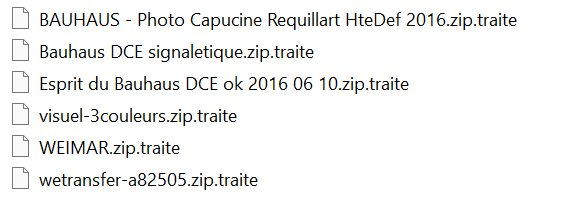
\includegraphics[width=0.8\textwidth]{Images/Decompression.jpeg}
	\caption{Vue rapprochée du renommage des archives compressées après exécution du script}
	\label{fig:Decompression}
\end{figure}

\textbf{Deuxième temps (tri et constitution d'un répertoire des éliminables)} : À partir de la croisée des données issues des exports de l'outil Droid, ce script effectue une opération chirurgicale sur les échantillons, il les nettoie et isole automatiquement les fichiers ou dossiers n'ayant aucun intérêt pour le fonds, notamment, les fichiers vides, temporaires, les doublons (à partir de la détection et la comparaison de l'empreinte numérique MD5) des fichiers sains.

\begin{figure}[H]
	\centering
	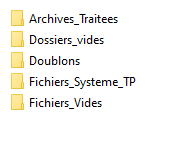
\includegraphics[width=0.8\textwidth]{Images/Arbo_Tri.PNG}
	\caption{Visualisation de l'arborescence de tri}
	\label{fig:Tri}
\end{figure}

\vspace{0.5cm} % Pour faire descendre le texte
\textbf{Troisième temps (transfert vers l'arborescence cible)} : Enfin, le troisième script parcourt les dossiers et fichiers sains qu'il transfère automatiquement l'arborescence institutionnelle de classement, c'est la fonction principale de notre traitement. À ce niveau, on peut se demander sur quelle base le transfert s'est opéré? La réponse est simple, l'algorithme reconstruit intégralement la structure du plan de classement. Pour rendre le transfert effectif, il se subdivise en deux points. Le premier se base sur une comparaison des synonymes qu'il récupère dans la colonne typologie, du dictionnaire de synonymes métiers en combinant au tri de surface (une comparaison avec le titre du fichier, à partir de l'héritage du dossier parent et les initiales des identifiants de la photothèque pour permettre l'identification d'images). Le second porte sur l'analyse sémantique textuelle pour les documents qui n'ont pas pu être traités en amont de l'opération. 

\begin{figure}[H]
	\centering
	\includegraphics[width=0.8\textwidth]{Images/Arbo-fichiers.png}
	\caption{Vue de l'arborescence de destination structurée générée automatiquement}
	\label{fig:Arborescence}
\end{figure}

 
Tout au long des différents transferts que nous avons effectué, la préservation des données est sécurisée par l'utilisation de la fonction de copie sécurisée : \textit{shutil.copy2()}. L'idée est de préserver les métadonnées d'origine des fichiers transférés, telles que la date de modification, les dates d'accès, les permissions. Toutefois, si l'algorithme rencontre un problème lié aux d'accès, il bascule en \textit{shutil.copyfile()}, qui copie le contenu des documents (date de création, auteur, date de modification, titre, etc.) qu'on retrouve généralement dans les détails des propriétés propres à ceux-ci. Ces données sont toutes aussi importantes pour assurer leur archivage pérenne. Nous avons eu l'exemple : Contenu créé : 18/07/2017 11: 30; ce qui représente la date d’origine de l’archive, inscrite directement dans la structure du document.

\section{Résultat et évaluation critique du traitement automatisé}

Une fois que nous avons appliqué les scripts à un ensemble réel, nous nous proposons dans cette partie de faire une analyse concrète sur le taux de réussite des différents scripts. Cette démarche se décline en deux parties : d'abord une évaluation quantitative, et ensuite une analyse des réussites ainsi que des erreurs.

\subsection*{Évaluation quantitative des trois étapes de traitement}

Nous détaillons notre analyse en trois temps :

\begin{table}[H]
	\centering
	\renewcommand{\arraystretch}{1.5}
	\setlength{\tabcolsep}{10pt}
	\resizebox{\textwidth}{!}{%
		\begin{tabular}{lrrr}
			\toprule
			\textbf{Dossier d'exposition} & \textbf{Nombre de fichiers} & \textbf{Archives décompressées} & \textbf{Taux de réussite} \\
			\midrule
			Cieslewicz-Expo & 21~980 & 100 & 100~\% \\
			French-touch    & 11~216 & 0   & --- \\
			Cartier2021     & 10~654 & 17  & 100~\% \\
			Bauhaus         & 15~284 & 468 & 100~\% \\
			\midrule
			\textbf{Total} & \textbf{59~134} & \textbf{585} & \textbf{100~\%} \\
			\bottomrule
		\end{tabular}%
	}
	\caption{Résultats de l'étape 1 -- décompression}
	\label{tab:etape1_decompression}
\end{table}


Le script parvient à appliquer correctement les trois temps de traitement sur les fichiers sélectionnés : détecter, décompresser et renommer.

\begin{table}[H]
	\centering
	\renewcommand{\arraystretch}{1.5}
	\setlength{\tabcolsep}{10pt}
	\resizebox{\textwidth}{!}{%
		\begin{tabular}{lrrrr}
			\toprule
			\textbf{Dossier d'exposition} & \textbf{Nombre de fichiers} & \textbf{Fichiers sains} & \textbf{Fichiers éliminables} & \textbf{Taux de réussite} \\
			\midrule
			Cieslewicz-Expo & 21~980 & 19~567 & 2~413 & 100~\% \\
			French-touch    & 11~216 & 5~026  & 6~190 & 100~\% \\
			Cartier2021     & 10~654 & 7~295  & 3~759 & 100~\% \\
			Bauhaus         & 15~284 & 7~117  & 8~167 & 100~\% \\
			\midrule
			\textbf{Total} & \textbf{59~134} & \textbf{39~005} & \textbf{20~529} & \textbf{100~\%} \\
			\bottomrule
		\end{tabular}%
	}
	\caption{Résultats de l'étape 2 -- tri}
	\label{tab:etape2_tri}
\end{table}

Comme le montre le tableau ci-dessus, l'algorithme parvient non seulement à écarter les fichiers sains des autres fichiers en les rangeant dans le dossier des éléments éliminables et les répartissant par catégories\footnote{Voir figure~\ref{fig:Tri}}.


\begin{table}[H]
	\centering
	\renewcommand{\arraystretch}{1.5}
	\setlength{\tabcolsep}{10pt}
	\resizebox{\textwidth}{!}{%
		\begin{tabular}{lrrr}
			\toprule
			\textbf{Dossier d'exposition} & \textbf{Correctement classés} & \textbf{Non classés} & \textbf{Taux de réussite} \\
			\midrule
			Cieslewicz-Expo & 19~471 & 96 & 99,51~\% \\
			French-touch    & 4~958  & 68 & 98,65~\% \\
			Cartier2021     & 7~285  & 10 & 99,86~\% \\
			Bauhaus         & 7~077  & 40 & 99,44~\% \\
			\midrule
			\textbf{Total} & \textbf{38~791} & \textbf{214} & \textbf{99,45~\%} \\
			\bottomrule
		\end{tabular}%
	}
	\caption{Résultats de l'étape 3 -- transfert vers l'arborescence cible}
	\label{tab:etape3_transfert}
\end{table}

Ici, l'algorithme arrive à transférer les fichiers sains retenus vers l'arborescence cible. Lors du test, nous avons constaté que le taux de réussite s'élève à 99,45~\%. Pour des raisons de sécurité, les fichiers non classés s'insèrent sous l'arborescence générée. Pour trouver le pourcentage de réussite par dossier racine traité, nous avons additionné le nombre de fichiers correctement classés par le nombre de fichiers non classés, puis divisé par le nombre de fichiers correctement classés et nous avons multiplié le résultat par 100.


\subsection*{Analyse quantitative des réussites, erreurs et écarts de catégorisation}

Les résultats mentionnés dans la section précédente nous interpellent et suscitent en nous quelques interrogations. D'abord, pourquoi y a-t-il un écart dans le traitement? Comme nous pouvons le voir, les deux premiers scripts fonctionnent à 100~\%, alors que le script de classement lui présente un taux de réussite moins élevé. Les deux premières opérations se déroulent bien tout simplement parce qu'elles se concentrent sur une analyse technique. Elles s'appuient uniquement sur les extensions de fichiers préalablement définis dans le fichier de configuration à partir de l'export Droid\footnote{Voir annexe~\ref{annexe:documentation-scripts}}. L’algorithme de transfert repose, quant à lui, sur une analyse beaucoup plus spécifique, à travers la comparaison des du contenu des fichiers. Ensuite, dans l'étape 3, pourquoi le taux d'erreurs varie selon le dossier racine? La logique de traitement ne dépend pas de la volumétrie du dossier à traiter, mais plutôt du nommage des fichiers traités et des résultats de l'analyse sémantique. Enfin, que deviennent les fichiers non classés? On remarque que 214 fichiers sur les 39 005 sains n'ont pas pu être classés. Ils sont donc rangés sous l'arborescence au même titre que les catégories du plan de classement. Cette logique peut sembler polluer l'arborescence, au contraire permet de faire un contrôle sur la qualité du traitement.

La phase d'expérimentation a nécessité plusieurs itérations algorithmiques, afin de corriger progressivement les limites techniques rencontrées lors de l'exécution des tests\footnote{Voir annexe ~\ref{annexe:journal-tests}}.

\section{Limites et conditions de poursuite du dispositif}

Cette partie dresse l'état des lieux des contraintes rencontrées sur le plan technique et des conditions requises pour assurer la pérennité de l'outil. Nous pouvons identifier la marge d'amélioration opérationnelle sans juger de la portée générale des résultats.


\subsection*{Limites techniques et méthodologiques révélées par l'expérimentation}

Cette analyse met en lumière des limites, liées aux phases de tri et d'arborescence. Premièrement, le traitement automatisé présente une anomalie : une copie du dossier des éliminables se crée dans l'arborescence du dossier racine, ce qui nécessite l'intervention humaine avant l'exécution du prochain script. Deuxièmement, le traitement physique de mise en arborescence des fichiers se heurte à des difficultés sémantiques. Le script ne classe pas les dossiers de manière uniforme, car le vocabulaire standardisé peut changer en fonction des expositions, et parce que nous n'avons pas adapté une structure de détection plus rigoureuse, compte tenu de la non uniformisation de la structure des documents en fonction de la typologie dans l'institution. 

\subsection*{Conditions de réutilisation et d’évolution du dispositif au sein du pôle Archives}

Afin de garantir l'utilisation pérenne de nos trois codes pour les archivistes du MAD, nous proposons une documentation qui explique les prérequis à mettre en place avant l’exécution jusqu'à leur application sur les dossiers d'exposition\footnote{Voir annexe~\ref{annexe:documentation-scripts}}. L'environnement de traitement dans lequel les programmes tournent est pensé pour permettre leur l'utilisation et leur compréhension par l'archiviste avec ou sans compétences techniques informatiques\footnote{Voir annexe~\ref{annexe:documentation-scripts}}. 
Cette approche permet aussi à travers les explications sur les éléments à renseigner dans le fichier de configuration. C'est aussi à ce niveau que nous montrons qu'il est important de prendre connaissance du vocabulaire de chaque exposition et renseigner dans la configuration\footnote{Voir annexe~\ref{annexe:documentation-scripts}}.\\[0.1cm]

En plus de la documentation, la réutilisation du dispositif repose sur la séparation entre le moteur de traitement et les règles métier, regroupées dans un même module de réglages. Celle-ci permet d'adapter le traitement à une nouvelle exposition, ainsi que de conformer le prototype à une éventuelle évolution des pratiques professionnelles. \\[0.1cm]

% Bout de code Python
\begin{lstlisting}[
	language=Python,
	captionpos=b,
	caption={Extrait du script de configuration \texttt{config.py}},
	label={lst:config}
	]
	# --- REGLAGES D'UNE NOUVELLE EXPOSITION ---
	dossier_racine = ""
	csv_file = "Export_Droid.csv"
	
	# Bareme des scores pour l'analyse semantique
	SCORE_MOT_CLE_TITRE = 90     # Mot-cle dans le nom du fichier
	SCORE_MOT_CLE_CONTENU = 30   # Mot-cle dans le texte
	SCORE_MAITRE_TITRE = 60      # Concept metier dans le titre
	SCORE_SYNONYME = 50          # Synonyme metier dans le titre
\end{lstlisting}


Le script complet de configuration est disponible dans le dépôt GitHub\footnote{Voir annexe~\ref{annexe:livrables-scripts-python}}. À partir de là, l'archiviste n'a pas besoin de modifier le corps de l'algorithme des scripts, il lui suffit juste d'ajouter de nouvelles variables dans le dossier de configuration.

